\documentclass[12pt]{article}

\usepackage[utf8]{inputenc}

\title{Rapid shortening at the eastern margin of the Tibetan plateau prior to the 2008 Mw=7.9 Wenchuan earthquake}
\author{T. Ben Thompson, Brendan J. Meade}
\date{September 2014}
\usepackage{graphicx}
\usepackage[margin=1.0in]{geometry}
\usepackage[nomarkers,figuresonly]{endfloat}
\usepackage{setspace}
\usepackage{natbib}
\doublespacing

\begin{document}

\maketitle

\section{Abstract}
The Longmen Shan is the steepest topographic front of the India-Asia collision and was the site of the Mw=7.9 Wenchuan earthquake. Shortening estimates across the Longmen Shan provide strain accumulation rates and clarify the eastward extrusion of the Tibetan plateau. Here, to explain the interseismic GPS velocities across the greater Longmen Shan region, we develop a boundary element model including earthquake cycle effects, topography, the westward dipping Beichuan fault, and a ~20 km deep, shallowly dipping, detachment. The detachment is inferred from observations of slip during and after the Wenchuan earthquake and from structural considerations. Previous analyses which neglected the detachment and earthquake cycle effects have found shortening rates near zero. In contrast, we find that interseismic GPS data are consistent with a shortening rate of 5.7$\pm$1.5 mm/yr. These results suggest that the Longmen Shan is an active fold-and-thrust belt with Wenchuan style earthquake recurrence intervals of $<$600 years.

\section{Introduction}
The Longmen Shan range is located on the eastern margin of the Tibetan and rises 5000m over 30km.  The 2008 $M_{\textrm{w}}$ 7.9 Wenchuan earthquake ruptured 250km along strike on the Beichuan and Pengguan faults, resulting in approximately 70000 fatalities. Prior geodetic estimates suggest almost zero horizontal shortening \citep{king97, chen00, shen05, Meade07c, Loveless2011}, in contrast with the dominant thrust slip-sense during the Wenchuan rupture.  Other authors reconcile the lack of shortening with the steep topography by appealing a lower crustal inflation tectonic model for the eastern Tibetan Plateau \citep{royden97, bird91, Burchfiel2008a}. However, the magnitude and location of the Wenchuan earthquake suggest a rapidly shortening fold-and-thrust belt. From seismic reflection data, \citet{hubbard09} find a well-developed fold-and-thrust fault system geometry with long-term shortenings up to 100\%. \citet{Fielding2012a} interpret satellite gravity-field data to infer that mass of the Longmen Shan is supported by a flexed Sichuan Basin. Seismic tomography, seismic reflection and magnetotelluric data have been used to suggest that this fold-and-thrust structure extends far into the plateau as a deep detachment \citep{Zhang2009, Zhao2012, Guo2013}. The Longriba fault zone, 200km northwest of the Longmen Shan, is suggested to also sole into this detachment \citep{Xu2008, Ren2013}.

However, it remains to be explained how slow present-day geodetic shortening estimates can be reconciled with the Wenchuan earthquake and the large structurally-observed shortening. Prior estimates can be categorized into those that neglect earthquake cycle effects, analyzing the fault slip-deficit without no explicit model of the geometry or tectonics, \citep{chen00, shen05} and those that use block models, which normally assume a simplified fault geometry \citep{Meade07c, Loveless2011, Burchfiel2008a}. \citet{Loveless2011} report the highest shortening rate of 3.2 mm/yr, as well as significant strain interior to the Longmen Shan block. Here, we present a model that includes earthquake cycle effects to explain the regional geodetic velocities as the result of a complex interseismically locked fault geometry, including a 20km deep detachment and the range-front Beichuan fault.  This geometry is consistent with the inference of 2-6m of slip of a 20km deep detachment that extends 90km northwest using InSAR measurements and post-Wenchuan GPS observations \citep{Qi2011}. \citet{Fielding2013b} also include a detachment fault plane in their joint geodetic-teleseismic coseismic slip inversion. Further, this geometry is suggested by structural interpretations \citep{Hubbard2010, Li2010}. Using this range-front thrust plus detachment geometry, we infer an average horizontal shortening between the TIbetan Plateau using interseismic GPS data collected prior to the Wenchuan earthquake.  Next, we show how this geometry can drive the steep velocity gradients far to the northwest of the range front, thus explaining the absence of a range-front interseismic velocity gradient. Importantly, this model provides increased estimates of seismic hazard. This model proposes that strain accumulates up to 300km from the margin of the Tibetan plateau while being released at the Longmen Shan range front, providing a unified theory of the Longmen Shan earthquake cycle. 

\section{Geodetic analysis of Longmen Shan shortening}

\begin{figure}[h!]
    \centering
    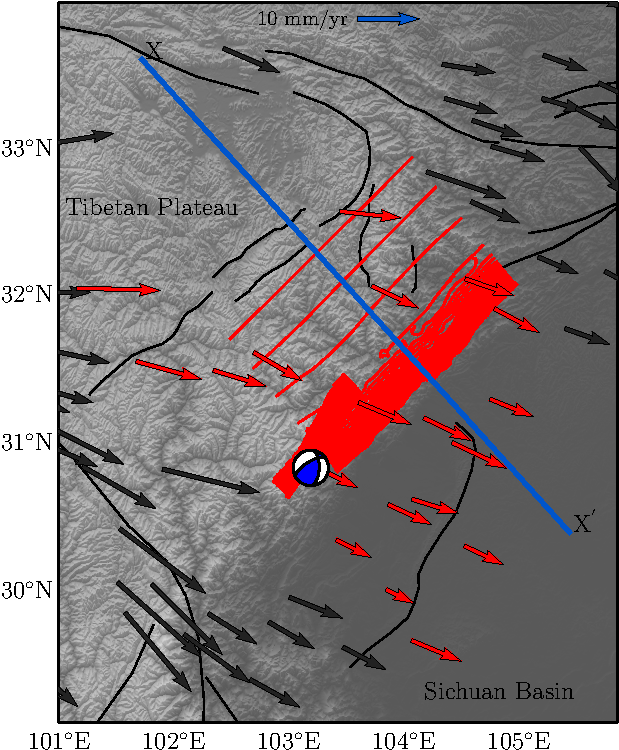
\includegraphics{figs/lms_map_all.pdf}
    \caption{A map of the Longmen Shan region with the basemap showing shaded relief. The focal mechanism plot is located at the epicenter of the Wenchuan earthquake, while the thicker red line shows the surface trace of rupture. The thin red lines show 1km depth contours of our model geometry. GPS velocity vectors are colored black if they are not included in our parameter estimation and red if they are included. The blue line shows the two-dimensional cross-section we study. Thin black lines indicate other significant faults in the region.}
    \label{fig:regional_map}
\end{figure}

The fault geometry we consider is derived from a community fault model for the Longmen Shan and Sichuan Basin region being actively developed (Plesch and Shaw, personal communication). This geometry is derived from structural interpretation of both seismic reflection surverys and surface geology \citep{Hubbard2010}. We make no modifications to this geometry except to take a fault-perpindicular cross-section. The depth and dip of the detachment are similar to the best-fitting surface found by \citet{Qi2011}. The cross-section and geometry with depth contours are shown in Figure \ref{fig:regional_map}. The fault geometry consists of two main segments. The range-front Beichuan fault dips steeply at ~60$^{\circ}$ at its surface trace shallowing to sub-horizontal near 20km depth where it joins the detachment surface at depth. The detachment dips at ~1.5$^{\circ}$ from an initial depth of 20km for 110km to the northwest at its deepest point with a depth of 23km.

Because this model includes a deep detachment, we must include interseismic GPS data far into the interior of the Tibetan Plateau. We study GPS observations collected prior to the Wenchuan earthquake \citep{apel06,Banerjee2008,calais06, gan07, vigny03}, assembled into a single reference frame by \citet{Loveless2011}. These velocities are shown in Figure \ref{fig:regional_map} along with the site of the Wenchuan earthquake and other regional faults \citep{Taylor09}. We include in the estimation velocities that are within the potential far-field influence of a deep detachment under the easternmost Tibetan Plateau. We exclude velocities that are near other major faults like the Xianshuihe fault or the Kunlun fault. Later, we demonstrate that our results are reasonably robust to the specific data set that is studied. Addition of more recent observations could bias our results due to possible postseismic transient deformation.

To analyze these data, we use a quasistatic elastic boundary element software under active development. An important feature of our tool is the inclusion of accurate surface topography in steep mountainous regions or Earth curvature in large-scale problems. In addition, we can accurately reproduce half-space solutions to very high precision. The steep topography of the Longmen Shan range front is included via the SRTM30\_PLUS digital elevation dataset \citep{Becker2009}. To maintain interseismic kinematic consistency between the Sichuan Basin and Tibetan Plateau, we use a 2D block formulation. The average interseismic slip-deficit on the fault geometry is subtracted from block motion to calculate the interseismic velocity profile (CITE?).

\begin{figure}[h!]
    \centering
    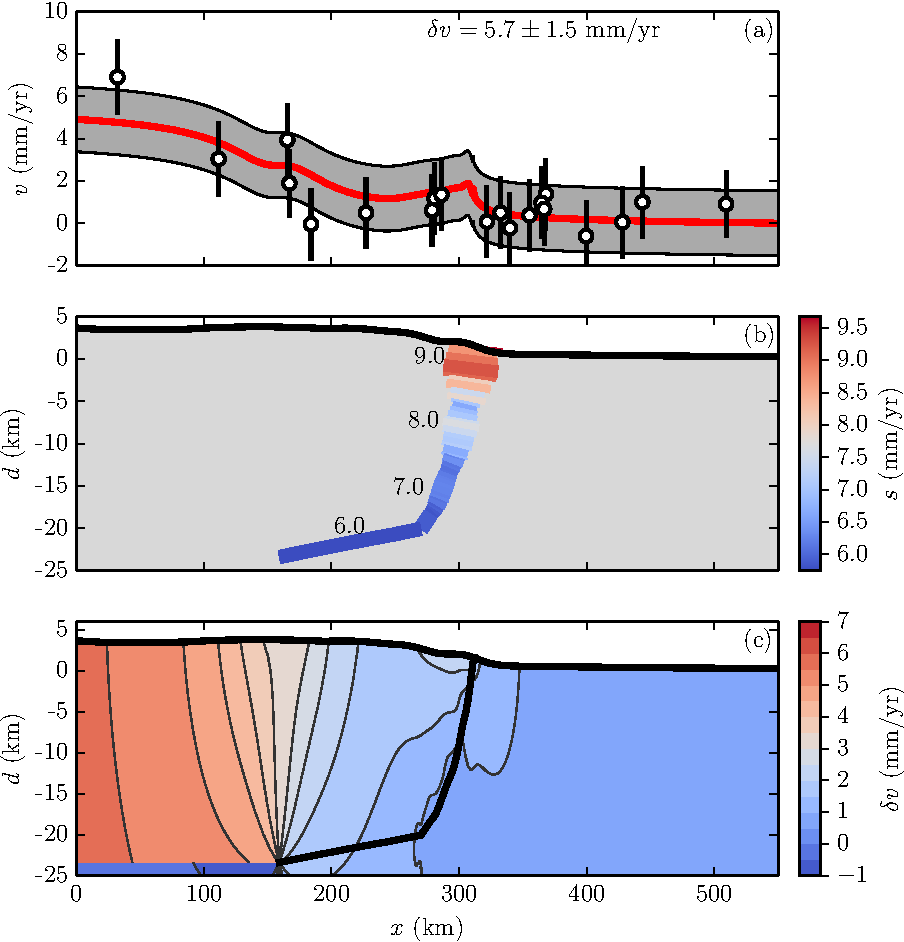
\includegraphics{figs/stack_figure_all_details.pdf}
    \caption{Axes are not one to one. a) Observed profile-parallel horizontal observed velocities are shown in black with 68\% confidence errorbars. Model-predicted velocities are shown by the red line with the surrounding gray region showing a 68\% confidence interval. b) Model geometry with colors and width along the locked fault showing predicted slip-deficit rates. Because shortening is the horizontal component of slip-deficit, increasing dips near the surface lead to larger slip-deficits. c) Predicted horizontal velocity as a function of depth. Note the steep velocity gradient and corresponding strain accumulation above the end of the detachment surface.}
    \label{fig:big_stack}
\end{figure}

The debate over shortening in the Longmen Shan has centered around the clear lack of an interseismic velocity gradient at the range front. However, this discussion has neglected the interplay between earthquake cycle effects and fault geometry. A Beichuan-only fault geometry would predict very little deformation beyond 100km \citep{savage83}, leading to the exclusion of velocities beyond this range. Both the observed and predicted profile-parallel velocities shown in Figure \ref{fig:big_stack}a make clear that such an estimate would result in a near-zero shortening estimate.

A locked detachment, however, drives the predicted location of steep velocity gradient far to the northwest as shown by Figure \ref{fig:big_stack}a. When including a locked detachment, the least squares best-fit shortening rate for the Longmen Shan region is 5.7 $\pm$ 1.5 mm/yr, a substantial increase over previous estimates. For discussion of seismic hazard, shortening must be translated to fault-parallel slip-deficit. Figure \ref{fig:big_stack}b shows the increase in slip-deficit from ~6.0 mm/yr up to 9.5 mm/yr at the surface. Figure \ref{fig:big_stack}c shows the horizontal velocities as a function of depth, demonstrating that the velocity gradients derive from the detachment tip. The smoothing behavior of an elastic Earth prevents distinguishing between a sharp drop in slip-deficit or a gradual change over many kilometers. These results demonstrate a mechanism by which it is possible for interseismic strain accumulation to occur far from the range-front structures on which it is released.

The primary uncertainty in our shortening estimate is the lack of good constraints on the detachment geometry in the hinterland. However, assuming the geometry is correct, two further forms of error are evident. First, the uncertainty in true interseismic velocities is propagated through to the estimated shortening, resulting in the gray region of uncertainty in Figure \ref{fig:big_stack}a. Further, the sparsity of observations suggests that certain observations may have undue influence on the shortening estimate. Excluding the northwest-most observation decreases the best-fit shortening to 3.9 $\pm$ 1.9 mm/yr. The least squares uncertainty is increased (from 1.5 mm/yr to 1.9 mm/yr) because the northwestern portion of velocities are poorly constrained once the observation is excluded. This northwestern-most observation is adjacent to the Longriba fault, suggesting that it should not be included. However, the Longriba fault is primarily a dextral strike-slip fault \citep{Ren2013}, so it's influence should be predominantly orthogonal to the profile parallel velocities we examine here.

Figure \ref{fig:distribution} shows a more complete analysis of the effect of case resampling the observations on the slip-deficit rate. Because there only $2^{20} = 1.048 $ million different possible subsets of the observations, we perform a complete case resampling bootstrap. Subsequently, we sample jointly from this distribution and the distribution of surface-area weighted fault depths. This analysis demonstrates that the majority of the slip-deficit-depth probability landscape lies at slip-deficit rates between 4 and 6 mm/yr while certain parts of the geometry (the range-front) have much faster slip-deficit rates. In Figure \ref{fig:distribution}, there is a non-negligible probability assigned to slip-rates above 10 mm/yr in the steepest, near-surface portion of the fault system. This is consistent with large near-surface coseismic slip during the Wenchuan earthquake \citep{Shen2009}. 

\begin{figure}[h!]
    \centering
    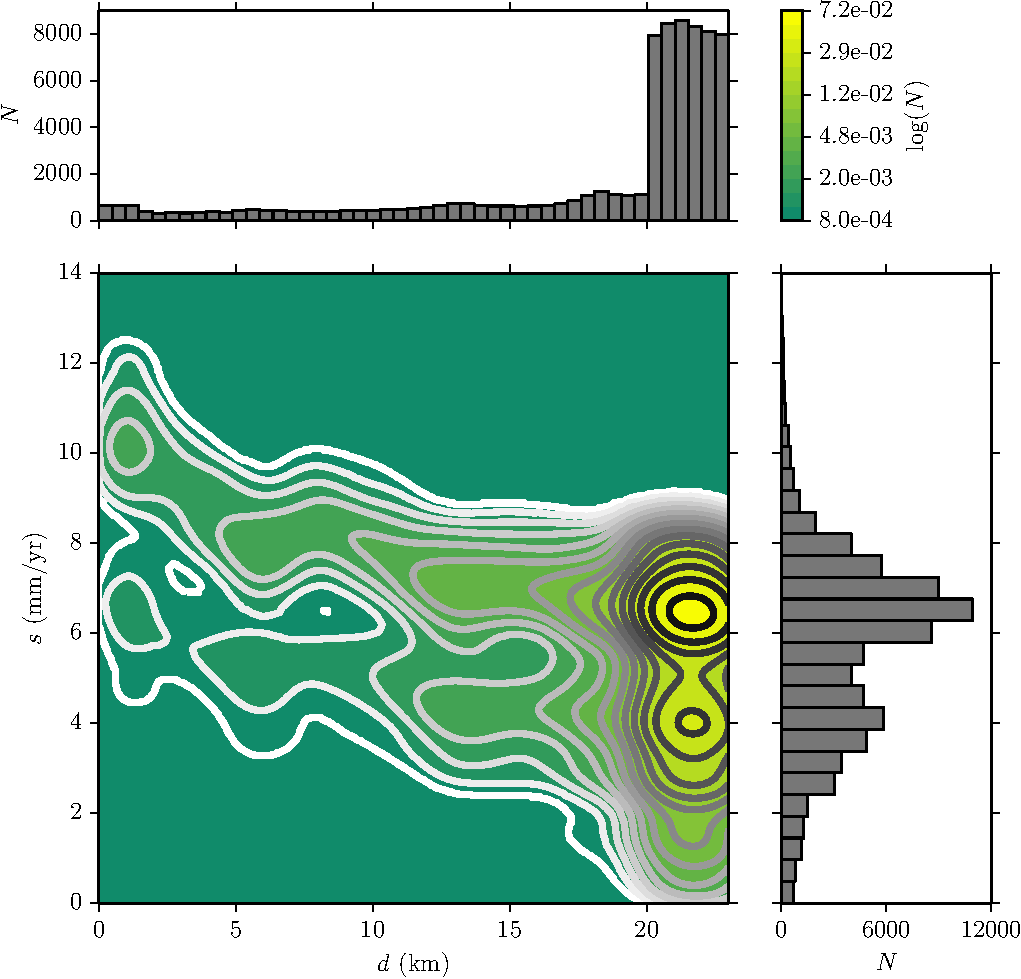
\includegraphics{figs/depth_slip_contour.pdf}
    \caption{The depth-slip-deficit probability landscape. The upper histogram is the projection of the contour plot onto a depth histogram, demonstrating that the majority of the fault surface area lies on the deep detachment. The right histogram is the projection of the contour plot onto a slip-rate histogram showing that the majority of fault surface area is slipping at rates near 6 mm/yr.}
    \label{fig:distribution}
\end{figure}

\section{Implications for the Longmen Shan earthquake cycle}
The striking feature of Figure \ref{fig:big_stack}a is the lack of a range-front geodetic signature despite the significant shortening rate. Locking on the deep detachment obscures the signal of deformation on the range-front faults. The interseismic deformation is much more broadly distributed across more than 300 kilometers. According to this model, interseismically, the eastern Tibetan Plateau moves cohesively with the Sichuan Basin, whereas coseismic slip is concentrated at the boundary between these two blocks.

\citet{Loveless2011} is the only prior geodetic model to include both a dipping Longmen Shan thrust and earthquake cycle effects. Compared to their estimated shortening rate of 3.2 mm/yr, our estimate is almost twice as large.  Their calculations show a comparatively high likelihood of internal block strain in the Longmen Shan region \citep{Loveless2011}. Attributing that block-internal strain to a deep detachment instead can explain the discrepancy between the two models. Our model of far-field deformation is also consistent with a similar detachment model of leveling and GPS-based uplift rates \citep{Hao2014}. The vertical velocities they measure increase from the Longmen Shan range front until peaking 50km southeast of the Longriba fault zone at approximately 3.5 mm/yr of uplift. The Longriba fault zone has the wrong slip-sense (thrusting up to the south-east, \citep{Ren2013}) to accomodate such vertical deformation. No other identified structures are nearby. 

The velocity gradient we attribute to a deep detachment has been attributed to broad viscous strain across the eastern Tibetan Plateau \citep{Royden2008}. Relatedly, \citet{kirby07} study an eastward decrease in interseismic velocities across the Kunlun fault. They conclude that the decline in slip-rate must be attributed to internal deformation. Further, fast erosion and inferred uplift rates have been used to support lower crustal inflation models in the absence of shortening \citep{Kirby2003}. All of these features can be explained with slip accomodated by a wide eastern Tibetan fold-and-thrust system, a suggestion supported by the continuation of shortening north from the Longmen Shan onto the Huya \citep{kirby00} and Min Jiang faults \citep{Chen1994}. In Figure \ref{fig:big_stack}c, broad strain is explained with long-term slip on a localized structure. Eastward declines in strike-slip motion on the major block-bounding faults can be explained by uplift and shortening accomodated across the eastern Tibetan Plateau. With growing evidence for long-term shortening, significant inferred erosion rates are no longer anomalous, being expected in a convergent setting. It is unknown how the demonstrated spatial decoupling of long-term fault slip from short-term interseismic uplift influences erosion. 

By the correspondence principle (cite), deep elastic fault motions and viscoelastic relaxation are difficult to distinguish without time-dependent data. The Wenchuan earthquake and significant observed afterslip on a deep detachment \citep{Qi2011, Huang2014} in the Longmen Shan support the detachment-based interpretation of eastern Tibetan Plateau tectonics. Similar to the Longmen Shan, low shortening rates have been observed on the Huya and Min Jiang fault \citep{Kirby2000}, in contrast to the $M_{\textrm{w}}$ 7.5 and 7.2 earthquakes in that region over the past century \citep{Chen1994}. It would be worthwhile to re-examine these shortening rates in the context of a detachment-based interpretation of the eastern Tibetan Plateau. 

We have not addressed when accumulated slip-deficit on the deep detachment is released. Postseismic slip incorporated in the model of \cite{Qi2011} shows up to 5 meters of slip on a deep detachment. Our data analysis depends on the detachment being locked during the period of data collection (when?). Aseismic slip may nonetheless be the predominant mode of strain release given the short observed portion of the earthquake cycle. Seismicity is approximately limited to the upper 20km of crust in the range-front \citep{Li2010}. Using steady-state critical taper wedge theory, we estimate a basal coefficient of friction between 0.02 and 0.30 for the detachment. The mean parameter estimate of 0.05 is comparable to estimates of friction on the low-angle detachment system beneath the Longmen Shan foreland \citep{Hubbard2010}, indicating a very weak fault over long time-periods. On the other hand, the surface area and shortening rate of the detachment could sustain very large earthquakes if slip is released coseismically. Specifically, if 100km down-dip and 300km along-strike were to slip 4 meters, similar to average slip during the Wenchuan earthquake, a $M_{\textrm{w}}$ 8.4 rupture would be produced.

As one of the first boundary element models to explicitly treat topography in crustal deformation analyses, it is interesting to ask which features of the predicted horizontal velocities are a result of topography. By comparing to a model without surface topography, the local minimum in velocity (Figure \ref{fig:big_stack}a) northwest of the Beichuan is identified as the main topographically-influenced feature. The effects may be more pronounced with a shallower fault dip like in a subduction zones. Despite the mediocre effect (~15\%), geodetic analyses in steep regions should consider topographic effects to avoid systematic bias.

Figure \ref{fig:hazard} shows a summary of recurrence intervals as a function of total event slip. Our shortening estimate suggests a recurrence interval for Wenchuan-like ruptures of approximately 600 years. Recurrence for smaller events is much more frequent. This contrasts with the average recurrence of ~2000 years determined by \citep{Ran2010} for the Beichuan fault. Our estimate would predict $M_{\textrm{w}} = $9.0 ruptures for that recurrence, seemingly unlikely given the total slip and fault length required. However, our estimate is an system-wide recurrence while paleoseismic estimates have been limited by only studying one of multiple imbricated thrusts. 

There are reasons to believe that the seismic hazard estimate presented here is a low estimate.  First, coseismic and long term slip estimates include a significant component of strike-slip motion\citep{Shen2009, Qi2011, Densmore2007} . But, we only model horizontal shortening. Second, our two-dimensional model assumes plane strain conditions. The approximation will result in under-estimates of the shortening required to produce far-field velocities. This is because the assumption is equivalent to assuming the fault geometry extends infinitely far along strike, a fault surface much larger than reality. Approximately 150 kilometers west of the Beichuan fault, there are 3 GPS stations with similar profile location. But, the velocities are significantly different. Hence, some lateral heterogeneity may not be represented by our two-dimensional modelling. This can also be seen in the shift of high topography from being SW-NE striking in the Longmen Shan to S-N striking in the adjacent Min Shan to north. Third, the modeled thrust is the steeply dipping Beichuan fault. The foreland Range Front thrust or the shallow detachment beneath Chengdu dip more shallowly \citep{Hubbard2010}, producing a greater total moment deficit.  Finally, the shortening rate estimate may be low due to being estimated late in the earthquake cycle \citep{savage00}.  It is also important that our recurrence interval calculation assumed the entire range-front was ruptured by the Wenchuan earthquake whereas the southern portion of the Longmen Shan did not rupture during the earthquake and is thought to similarly active to the portions that did rupture \citep{Li2010}. 


\begin{figure}[h!]
    \centering
    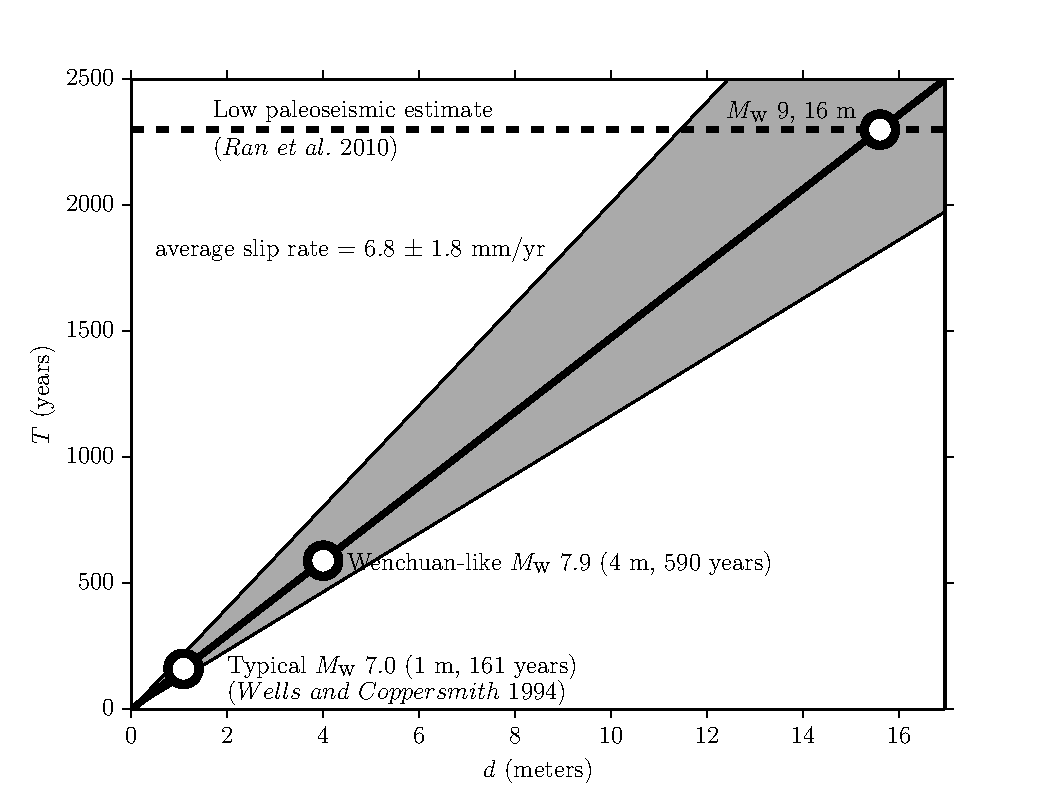
\includegraphics{figs/hazard_all_details.pdf}
    \caption{Recurrence as a function of slip, assuming the best-fit slip rate for the Beichuan fault. The gray region indicates the uncertainty implied by the error in our shortening estimate. The discrepancy between the Wenchuan-like recurrence and the paleoseismic estimate may be due to the presence of multiple active faults in the range-front.}
    \label{fig:hazard}
\end{figure}

\section{Conclusion}
Previous near-zero shortening estimates in the Longmen Shan are at odds with the large-moment of the Wenchuan earthquake, very steep topography, structural interpretations indicate fold-and-thrust geometry, fast erosion rates. We clarify this conflict by including earthquake cycle effects and a 20km deep detachment. Our revised interseismic shortening rate is 5.7 $\pm$ 1.5 mm/yr with fault slip-deficit rates up to 9.5 mm/yr near the surface, where the Beichuan fault is steepest. The model shows that interseismic strain accumulation may be spatially disjoint with coseismic strain release, emphasizing that accurate fault geometries are critical in the analysis of geodetic data. This interpretation unifies geodetic models of coseismic, postseismic and interseismic crustal deformation in the Longmen Shan. Finally, our model suggest that Wenchuan-like events have much shorter recurrence intervals.

\bibliographystyle{plainnat}
\bibliography{biblio,library}
\end{document}
